%%%%%%%%%%%%%%%%%%%%  BUSINESS EMAIL COMPROMISE %%%%%%%%%%%%%%%%%%%%
\newpage
\subsection{Business Email Compromise}
\subsubsection{Lower Bound Computation}
\[
\begin{bmatrix}
\mathbf{x}_{\text{American Samoa}}^{(\text{count})}\\
\mathbf{x}_{\text{American Samoa}}^{(\text{dollars})}
\end{bmatrix}
=
\begin{bmatrix}
0 & 0 & \cdots & 2\\
\$0 &\$0 & \cdots &\$960 
\end{bmatrix}.
\]
\[
\begin{bmatrix}
\mathbf{x}_{\text{American Samoa}}^{(\text{count scaled to sample population})}\\
\mathbf{x}_{\text{American Samoa}}^{(\text{dollars scaled to sample population})}
\end{bmatrix}
=
\begin{bmatrix}
0 & 0 & \cdots & 8\\
\$0 & \$0 & \cdots &\$3{,}360
\end{bmatrix}.
\]
  \[
\bar{X}_{\text{American Samoa}}^{(m)}
= \frac{1}{N}\sum_{i=1}^{N} X_{\text{American Samoa},i}^{(m)},
\]
\\
\[
\qquad
m \in \{\text{scaled count},\text{scaled dollars}\}
\]
\[
\begin{bmatrix}
\bar{X}_{\text{American Samoa}}^{(\text{scaled count})}\\
\bar{X}_{\text{American Samoa}}^{(\text{scaled dollars})}
\end{bmatrix}
=
\begin{bmatrix}
4\\
\$13{,}851
\end{bmatrix}.
\]
\subsubsection{Upper Bound Computation}
\[
\begin{bmatrix}
\mathbf{x}_{\text{California}}^{(\text{count})}\\
\mathbf{x}_{\text{California}}^{(\text{dollars})}
\end{bmatrix}
=
\begin{bmatrix}
2{,}155 & 2{,}429 & \cdots & 3{,}269\\
\$69{,}208{,}381 &\$106{,}225{,}791  & \cdots &\$439{,}425{,}357 
\end{bmatrix}.
\]
\[
\begin{bmatrix}
\mathbf{x}_{\text{California}}^{(\text{count scaled to sample population})}\\
\mathbf{x}_{\text{California}}^{(\text{dollars scaled to sample population})}
\end{bmatrix}
=
\begin{bmatrix}
9 & 11 & \cdots & 15\\
\$289{,}037 &\$481{,}055 & \cdots &\$2{,}016{,}329 
\end{bmatrix}.
\]
\[
\bar{X}_{\text{California}}^{(m)}
= \frac{1}{N}\sum_{i=1}^{N} X_{\text{California},i}^{(m)},
\]
\\
\[
\qquad
m \in \{\text{scaled count},\text{scaled dollars}\}
\]
\[
\begin{bmatrix}
\bar{X}_{\text{California}}^{(\text{scaled count})}\\
\bar{X}_{\text{California}}^{(\text{scaled dollars})}
\end{bmatrix}
=
\begin{bmatrix}
13\\
\$784{,}561
\end{bmatrix}.
\]
\subsubsection{Monte Carlo Simulations for Likelihood and Impact}
\begin{figure}[H]
  \centering
  \rotatebox{0}{\scalebox{1}{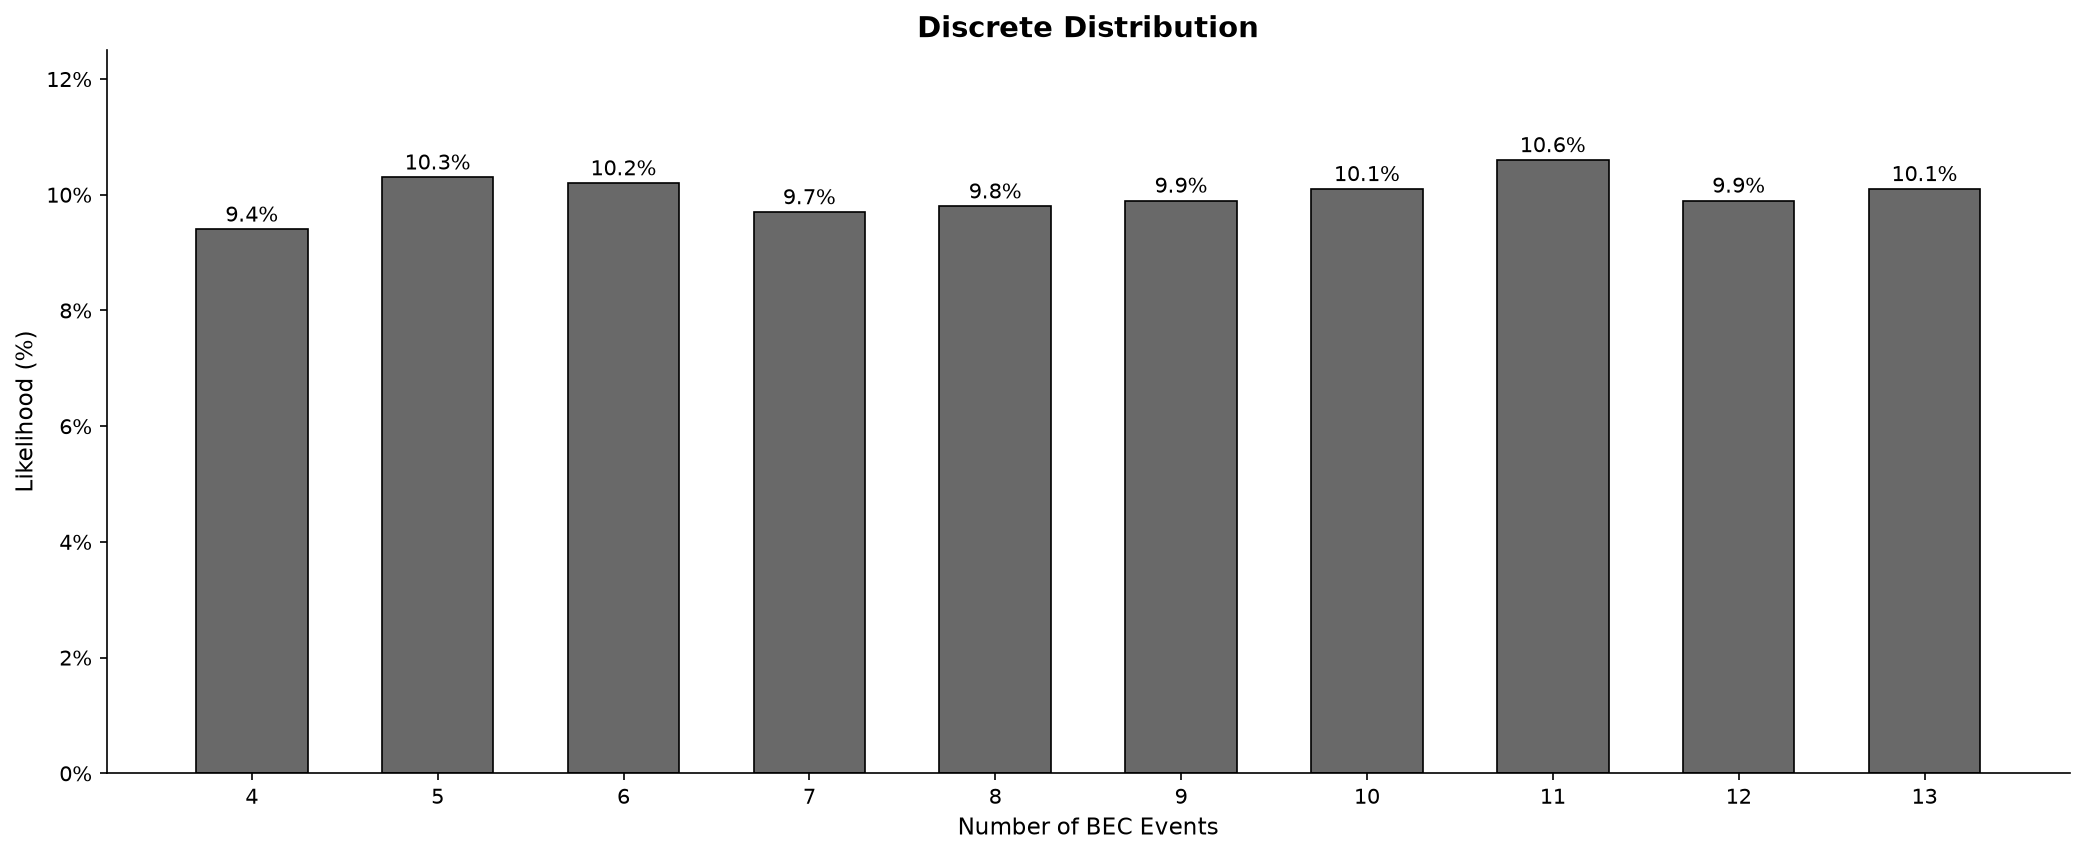
\includegraphics[scale=0.25]{figures/discrete_bec_count.png}}}
  \caption{We ran a\index{Monte Carlo simulation} Monte Carlo simulation of 10,000 iterations with a discrete distribution to spread random instances between confidence intervals taken from the means of seven year samples. We bounded between 4 and 13 possible \index{business email compromise}business email compromise events over a year.\protect\endnote{\index{sample} Sample size was set equivalent to the City of\index{Chattanooga} Chattanooga to determine the per capita rates for each year over data from \index{American Samoa} American Samoa and\index{California} California.  The means of those rates were used to set lower and upper bounds with \index{American Samoa} American Samoa and\index{California} California representing low and high \index{cybercrime} cybercrime counts respectively.}
  \protect\endnote{Monte Carlo Modeling Toolkit authored by Derek E. Brink, CISSP, \url{www.linkedin.com/in/derekbrink}. March 2023.}
  }
  \label{fig:screenshot-montecarlo-bec-count-discrete}
\end{figure}
When we computed the upper and lower bounds, we recognized that a normal distribution would not fit well for forecasting likelihood.  We took the mean of the sample from American Samoa for the lower bound (4); we took the mean from the sample from California for the upper bound (13); we had a separation of 9 units.  Therefore, we switched to a discrete model with all 10 options sharing an equal likelihood.
\begin{table}[H]
  \centering
  \caption{Monte Carlo Discrete Simulation Values for Business Email Compromise}
  \label{tab:discrete_bec_montecarlo}
  \begin{center}
  \begin{tabular}{@{}>{\centering\arraybackslash}
  p{0.20\linewidth} >{\centering\arraybackslash}
  p{0.10\linewidth}>{\centering\arraybackslash}
  p{0.10\linewidth}>{\centering\arraybackslash}
  p{0.10\linewidth}>{\centering\arraybackslash}
  p{0.10\linewidth}>{\centering\arraybackslash}  
  p{0.10\linewidth}}
    \toprule
Events
&4
&5
&6
&7
&8\\
    \midrule
Likelihood    
&9.4\%
&10.3\%
&10.2\%
&9.7\%
&9.8\%\\
    \bottomrule \end{tabular}
\begin{tabular}{@{}>{\centering\arraybackslash}
  p{0.20\linewidth} >{\centering\arraybackslash}
  p{0.10\linewidth}>{\centering\arraybackslash}
  p{0.10\linewidth}>{\centering\arraybackslash}
  p{0.10\linewidth}>{\centering\arraybackslash}
  p{0.10\linewidth}>{\centering\arraybackslash}
  p{0.10\linewidth}}
    \toprule
Events    
    &9
    &10
    &11
    &12
    &13\\
    \midrule
Likelihood
&9.9\%
&10.1\%
&10.6\%
&9.9\%
&10.1\%\\
    \bottomrule \end{tabular}
    \end{center}
  \raggedright{A\index{Monte Carlo simulation} Monte Carlo simulation was run using a discrete distribution.  We bounded the simulation between 4 and 13 events.  We assigned a 10\% likelihood to each bin.  The resulting distribution showed the effect of randomness on each possible outcome.}
\end{table}

\begin{figure}[H]
  \centering
  \rotatebox{0}{\scalebox{1}{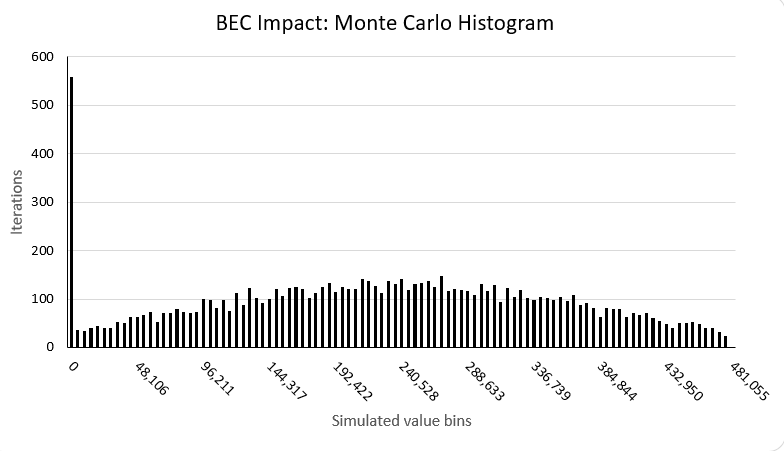
\includegraphics[width=\linewidth]{figures/histogram_bec_impact.png}}}
  \caption{We ran a\index{Monte Carlo simulation} Monte Carlo simulation of 10,000 iterations with a normal distribution to spread random instances between bounds taken from means of seven year samples. We set a lower bound that the events would cost at \$0.  We set an upper bound that the events would cost \$784{,}561.  \protect\endnote{\index{sample} Sample size was set equivalent to the City of\index{Chattanooga} Chattanooga to determine the per capita rates for each year over data from \index{American Samoa} American Samoa and\index{California} California.  The means of those rates were used to set upper and lower bounds with \index{American Samoa} American Samoa and\index{California} California representing low and high \index{cybercrime} cybercrime counts respectively.}
  \protect\endnote{Monte Carlo Modeling Toolkit authored by Derek E. Brink, CISSP, \url{www.linkedin.com/in/derekbrink}. March 2023.}
  }
  \label{fig:screenshot-montecarlo-bec-impact-histo}
\end{figure}
\begin{figure}[H]
  \centering
  \rotatebox{0}{\scalebox{1}{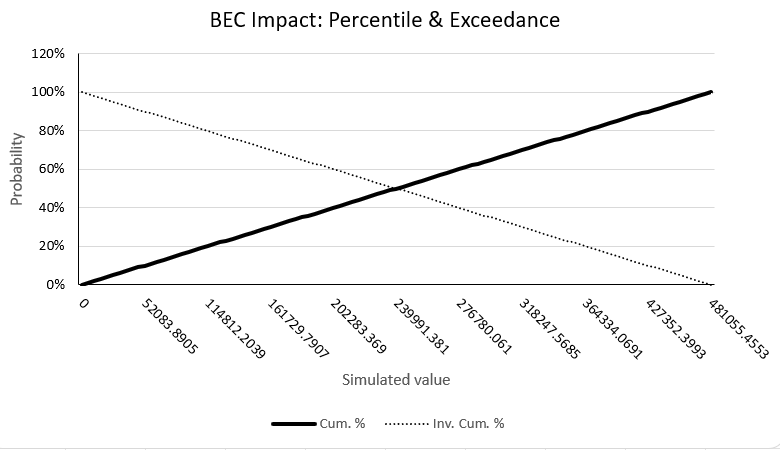
\includegraphics[width=\linewidth]{figures/percent_bec_impact.png}}}
  \[
\mathrm{CI}_{80\%}(\theta) = [\$78{,}456, \$706{,}105]
\]
  \caption{A\index{Monte Carlo simulation} Monte Carlo simulation with a normal distribution suggests that there is a 90\% probability that\index{business email compromise} business email compromise events will cost \$78{,}456 or more in a year.  There is a 50\% likelihood that they will cost \$392{,}281 or more in a year.  There is a 10\% chance that they will cost \$706{,}105 or more in a year. \protect\endnote{\index{sample} sample size was set equivalent to the City of\index{Chattanooga} Chattanooga to determine the per capita rates for each year over data from \index{American Samoa} American Samoa and\index{California} California.  The means of those rates were used to set lower and upper bounds with \index{American Samoa} American Samoa and\index{California} California representing low and high \index{cybercrime} cybercrime impact values respectively.}
  \protect\endnote{Monte Carlo Modeling Toolkit authored by Derek E. Brink, CISSP, \url{www.linkedin.com/in/derekbrink}. March 2023.}
  }
  \label{fig:screenshot-montecarlo-bec-impact-percent}
\end{figure}

% =========================================================================
% DATA NOTES (not for typesetting — reference documentation)
% =========================================================================
% Source workbook: ComputerCrime_AUG2026_Impact_Final_With_C5C7_IFERROR_CHARTS_FIXED.xlsx
% Workbook now contains a Discrete_BEC sheet (added programmatically).
%
% AMERICAN SAMOA BEC (years selected: 2016, 2017, 2022)
%   Raw counts:          2016=0, 2017=0, 2022=2
%   Raw state losses:    2016=$0, 2017=$0, 2022=$960
%   Scaled counts:       2016=0, 2017=0, 2022≈8 (7.616)
%   Scaled impacts:      2016=$0, 2017=$0, 2022=$3,360
%   All 7 year mean scaled count:  (0+0+0+0+18+3+8)/7 = 4.09 ≈ 4
%   All 7 year mean scaled impact: (0+0+0+0+0+93600+3360)/7 = $13,851
%
% CALIFORNIA BEC (years shown: 2016, 2017 ... 2022)
%   Raw counts:          2016=2,155  2017=2,429 ... 2022=3,269
%   Raw state losses:    2016=$69,208,381  2017=$106,225,791 ... 2022=$439,425,357
%   Scaled counts:       2016=9  2017=11 ... 2022=15
%   Scaled impacts:      2016=$289,037  2017=$481,055 ... 2022=$2,016,329
%   All 7 year mean scaled count:  (9+11+13+16+13+13+15)/7 = 12.86 ≈ 13
%   All 7 year mean scaled impact: $784,561
%
% MONTE CARLO BOUNDS
%   Lower bound (American Samoa mean): 4
%   Upper bound (California mean):    13
%   Separation: 9 units, 10 options (4 through 13)
%   Assigned likelihood per bin: 10% each
%
% DISCRETE SIMULATION (10,000 iterations, seed=42, discrete uniform 4-13)
%   4: 944  (9.4%)   5: 1032 (10.3%)   6: 1016 (10.2%)
%   7: 969  (9.7%)   8: 982  (9.8%)    9: 986  (9.9%)
%  10: 1014 (10.1%)  11: 1056 (10.6%)  12: 989  (9.9%)  13: 1012 (10.1%)
%
% IMPACT MONTE CARLO (uniform distribution, lower=$0, upper=$784,561)
%   10th pct (cost >= 90% of time):  $78,456
%   50th pct (cost >= 50% of time):  $392,281
%   90th pct (cost >= 10% of time):  $706,105
%   80% CI: [$78,456, $706,105]
% =========================================================================
